To bridge between the desired $x$-space input/output and the internal
Mellin representation, we do a Lagrange-Interpolation as sketched in
\cref{sec:theory:interpolation}
(and detailed in the \href{https://eko.readthedocs.io/en/latest/}{online documentation}).
We recommend a grid of at least 50 points with
linear scaling in the large-$x$ region ($x \gtrapprox 0.1$) and with logarithmic
scaling in the small-$x$ region and an interpolation of degree four.
Also the grids determined by \amcfast~\cite{Bertone:2014zva} perform
sufficiently well for specific processes.

\begin{figure}
    \begin{center}
    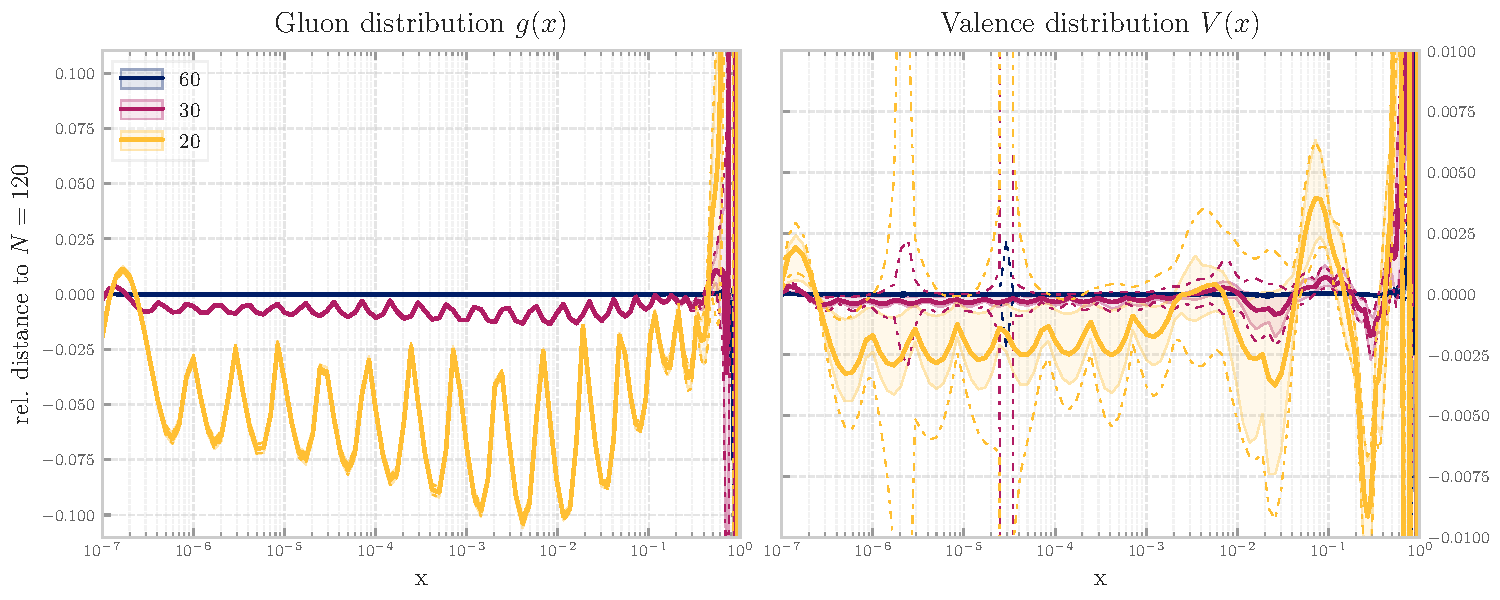
\includegraphics[width=\textwidth]{ch-eko/interpolation-int-ratio}
    \end{center}
    \caption{Relative differences between 
        the outcome of \nnlo{} \qcd{} evolution
        as implemented in \eko{} with 20, 30, and 60 points to 120
        interpolation points respectively.
        \label{fig:interpolation} }
\end{figure}

For a first qualitative study we show in \cref{fig:interpolation} a
comparison between an increasing number of interpolation points
distributed according to \cite[Eq. 2.12]{Carrazza_2020}.
The separate configurations are converging to the solution with the
largest number of points. Using 60 interpolation points is almost
indistinguishable from using 120 points (the reference configuration in the plot).
In the singlet sector (gluon) the convergence is
significantly slower due to the more involved solution strategies and,
specifically, the oscillating behavior is caused due to these difficulties.
The spikes for $x\to 1$ are not relevant since the \pdfs are intrinsically
small in this region ($\vb f\to 0$) and thus small numerical differences
are enhanced.

Also note that the results of \cref{sec:pheno:bench} (i.e.\ \cref{fig:LHAbench,fig:Apfelbench_pto,fig:Pegasusbench_pto}) confirm that
the interpolation error can be kept below the benchmark accuracy.
